\documentclass[anonymous,timestamp,review,acmtog]{acmart}

\usepackage{booktabs} % For formal tables
%\usepackage{subfigure}
\usepackage{subcaption}
\usepackage{graphicx}
%\graphicspath{{C:/Users/black/OneDrive/Documents/UT/Research/Shell/MoistInducedSim}}

\newcommand{\ba}{\mathbf{a}}
\newcommand{\bb}{\mathbf{b}}
\newcommand{\bc}{\mathbf{c}}
\newcommand{\bg}{\mathbf{g}}
\newcommand{\br}{\mathbf{r}}
\DeclareMathOperator{\tr}{tr}
\newcommand{\hn}{\hat{\mathbf{n}}}

\acmPrice{15.00}

% The next six lines come directly from the completed rights form.
% You MUST replace them with the lines specific to your accepted work.
\copyrightyear{2018}
\acmYear{2018}
\setcopyright{rightsretained}
\acmConference{Conference Name}{Conference Date and Year}{Conference Location}
\acmDOI{10.1145/8888888.7777777}
\acmISBN{978-1-4503-1234-5/17/07}

% Use the "authoryear" citation style, and make sure citations are in [square brackets].
\citestyle{acmauthoryear}
\setcitestyle{square}

% A useful command for controlling the number of authors per row.
% The default value of "authorsperrow" is 2.
\settopmatter{authorsperrow=2}

% end of preamble.

\begin{document}

% Title. 
% If your title is long, consider \title[short title]{full title} - "short title" will be used for running heads.
\title{Physical Simulation of Moisture Induced Thin Shell Deformation}

% Authors.
\author{Hsiao-yu Chen}
\affiliation{%
  \institution{University of Texas at Austin}}

\author{Etienne Vouga}
\affiliation{%
  \institution{University of Texas at Austin}}

% This command defines the author string for running heads.
%\renewcommand{\shortauthors}{DeJohnette, Rowland-Smith, Badeeri, and Foyt}

% abstract
\begin{abstract}

\end{abstract}

%CCS
\begin{CCSXML}
%<ccs2012>
%<concept>
%<concept_id>10010147.10010371.10010372</concept_id>
%<concept_desc>Computing methodologies~Rendering</concept_desc>
%<concept_significance>500</concept_significance>
%</concept>
%<concept>
%<concept_id>10010147.10010371.10010372.10010374</concept_id>
%<concept_desc>Computing methodologies~Ray tracing</concept_desc>
%<concept_significance>500</concept_significance>
%</concept>
%</ccs2012>
\end{CCSXML}

%\ccsdesc[500]{Computing methodologies~Rendering}
%\ccsdesc[500]{Computing methodologies~Ray tracing}
%
%%keywords
%\keywords{ray tracing, global illumination, octrees, quadtrees}
%
%% A "teaser" figure, centered below the title and authors and above the body of the work.
%\begin{teaserfigure}
%  \centering
%  \includegraphics[width=6.0in]{aaafiles/fountain}
%  \caption{Drumheller Fountain, The University of Washington, Seattle WA.}
%\end{teaserfigure}
%
%% Processes all of the front-end information and starts the body of the work.
\maketitle

\section{Introduction}


\paragraph{Contribution} We present a low-order discrete shell model tailored to simulating non-unform, anisotropic, differential swelling and shrinking of thin shells. In contrast to previous methods for simulating related phenomena, such as burning and growth, our formulation builds on discrete geometric shell theory and supports arbitrary rest curvature and strain, and physical settings such as thickness and Lam\'{e} parameters. We couple our shell model to a simple formulation of moisture diffusion in both the lateral and thickness directions, which takes into account anisotropy of the material grain. In a series of experiments, we show that our model successfully predicts the qualitative behavior of thin shells undergoing complex, dynamic deformations due to swelling or shrinking, such as occurs when paper is moistened, leaves dry in the sun, or thin plastic melts.

\subsection{Related Work}
\paragraph{Simulating Burning/Melting/Swelling} Several papers look at related problems, such as evolving the boundary of a burning or melting solid, without incorporating curling/wrinkling and other elastic deformations of the solid. Melek and Keyser~\shortcite{Melek2003,Melek2005} simulate pyrolysis and heat diffusion of burning objects, but do not consider elastic deformation of the burning objects. Losasso et al~\shortcite{Losasso2006} proposed tracking of the burning boundary of thin shells using an adaptive level set on the shell. Some of the deformation can be qualitatively approximated by mapping physical quntities like heat and moisture to cells of a coarse grid around the object, deforming the cage, and mapping the deformation back onto the shell (as in Free Form Deformation); this approach was proposed by Melek and Keyser~\shortcite{Melek2007} and adopted by Liu et al~\shortcite{Liu2009}. Most similar to our work is the method of Jeong et al~\shortcite{Jeong2011,Jeong2013}, which uses a \emph{bilayer} of springs (a triangle mesh and its circumcentric dual, offset a distance from the primal mesh) to represent the shell. The bilayer allows the method to capture \emph{differential} growth due to gradients in moisture concentration across the thickness of leaves, leading to visually impressive simulations of leaves curling as they dry. Our work is based on the same fundamental idea (representing the shell using rest geometry that varies linearly through the thickness) but couched in the machinery of differential geometry; our formulation allows us to easily incorporate non-zero rest curvature, machine direction, and a physical material model.

Steps towards a principled physical model include the use of a mass-spring network to represent the shell, with update rules for how spring rest lengths should change due to physical processes in the shell. Such rules are simplest to formulate in the case where growth or shrinkage is uniform through the shell thickness, and the shell can be represented using a single spring layer; Larboulette et al~\shortcite{Larboulette2013} present such a rule, which includes handling of the \emph{machine direction} of paper: a bias in the orientation of the fibers composing the paper which causes the paper to swell anisotropically. We adopt this parameter in our material model. 

\paragraph{Mechanics of Shells}
The mathematics and geometry underpinning the physics of thin shells is a venerable topic: Ciarlet's book~\shortcite{Ciarlet2000} on elasticity as applied to shells offers a thorough overview. Our work is based on the common \emph{Kirchhoff-Love} assumption that the shell does not undergo any transverse shear; ie, that the shell volume is foliated by normal offsets of the shell's \emph{midsurface}: the problem of studying deformation of the 3D shell volume then reduces to that of deformation of a 2D surface, and tools from Riemannian geometry can be applied. (We adopt the so-called ``intrinsic'' view~\cite{Neff2004} that shells can be understood in terms of Kirchhoff-Love and geometric principles, as this view allows us to easily discretize shell physics by leveraging discrete differential geometry, but we note in passing that the validity of the Kirchhoff-Love assumption, and of reduced shell models in general, remains unsettled, and the literature documents numerous alternative shell theories.) One key property of the shells we want to simulate is that they are \emph{non-Euclidean}: they do not have a rest (strain-free) state that is realizable in three-dimensional space. Non-Euclidean shells have received substantial attention recently in the physics community~\cite{Klein2007,Kim2012}, thanks to their potential applications in fabrication and robotics, and their connection to biological growth; Sharon and Efrati~\cite{Efrati2009,Sharon2010} pioneered the study of shell mechanics in this setting.

For the sake of being self-contained, we briefly review the geometric foundations of shell mechanics in Section \ref{sec:continuous}.

\paragraph{Computational Modeling of Thin Shells} 
Thin shells first caught the interest of the graphics community in the context of simulating cloth~\cite{Baraff1998,Bridson2002}. These early methods tended to focus on thin \emph{plates}, i.e. shells that are rest flat, and formulate shell dynamics either in terms of either hinge-based bending energies~\cite{Sullivan2008,Tamstorf2013} or the insight that the bending energy can be written in terms of the intrinsic Laplace-Beltrami operator applied to the shell's embedding function~\cite{Bobenko2005,Bergou2006,Wardetzky2007}. Grinspun et al~\shortcite{Grinspun2003} introduced to graphics the simulation of shells with non-flat rest curvature. Their formulation is based on \emph{differences of squared mean curvature}, leading to a simple and easy-to-discrete bending energy; this model is physically suspect, however: consider a half-cylinder at rest when curled around the $x$-axis. Unbend the shell and re-bend it around the $y$-axis; the deformed configuraiton's strain cannot be captured by looking at mean curvature alone, as it is pointwise identical to the mean curvature of the rest configuration. Complete support for rest curvature requires a bending energy that incorporates full information about the extrinsic deformation of the shell~\cite{Grinspun2006}. One recent such discrete energy is described in Weischedel's under-appreciated work on discrete Cosserat shells~\shortcite{Weischedel2012}; our exposition is modeled closesly on hers, though we make different modeling choices (we use an intrinsic rather than Cosserat shell model, and require more flexible handling of the shell rest geometry).

Higher-order methods for simulating shells (including with e.g. NURBS or subdivision elements) are common in computational mechanics and isogeometric analysis~\cite{Cirak2000,Kiendl2009,Benson2010,Bandara2018} and have also been proposed for computer graphics~\cite{Wawrzinek2011}. High-order methods have some obvious advantages (better convergence behavior in the thin limit, especially for shell deformations involving large strains; continuous surface normals) at the cost of additional computational cost and complexity, especially when handling contact.

In this paper, we ignore the problem of mesh tesselation, or of adapting the mesh in response to either large deflections or large amounts of growth; such remeshing is an important component of a practical shell simulation but orthogonal to our focus on shell dynamics. ArcSim~\cite{Narain2012} incorporates a method of adaptive remeshing while avoiding significant popping artifacts, and has been used to generate impressive simulations of creasing paper. Vetter et al~\shortcite{Vetter13} study the companion problem of remeshing due to large in-plane growth, and present a solution based on adaptive Loop subdivision.

\section{Continuous Formulation} \label{sec:continuous}
Before describing our discretization of shells, we briefly review the formulation in the continuous setting, as this formulation will guide our discretization. 

\paragraph{Shell Geometry} We can represent shells $S\subset \mathbb{R}^3$ of thickness $h$ by a parameter domain $\Omega$ in the plane and an embedding $\phi: \Omega\times [-h/2, h/2]\to\mathbb{R}^3$ with $S$ the image of $\phi$ (see Figure~\ref{fig:XXX}). We adopt the common \emph{Kirchhoff-Love} assumption that the shell does not undergo any transverse shear; ie, that the shell volume is foliated by normal offsets of the shell's \emph{midsurface} $\br:\Omega\to\mathbb{R}^3$. In other words,
$$\phi(x,y,z) = \br(x,y) + z\hn(x,y)$$
where $\hn = (\br_x \times \br_y)/\|\br_x \times \br_y\|$ is the midsurface normal. The shell's deformation is thus completely determined by the deformation of the midsurface. The metric $\bg$ on the slab $\Omega \times [-h/2,h/2]$, pulled back from $\mathbb{R}^3$, can be expressed in terms of the geometry of the midsurface:
$$\bg = \left[\begin{array}{cc}\ba - 2z\bb + z^2 \bc & 0\\0 & 1\end{array}\right],$$
where
$$\ba = d\br^Td\br \quad \bb = -d\br^Td\hn \quad \bc = d\hn^Td\hn$$
are the classical first, second, and third fundamental forms of the surface $\br$.

Oftentimes, the parameterization domain of a thin shell is assumed to be also the rest state of the shell, so that the strain in the material of the shell can be determined directly from looking at $\bg$. We cannot assume this: consider for instance a piece of paper whose center has been moistened by spilled coffee. The fibers in the coffee stain stretch; since they are confined by the surrounding non-wet region of the paper, the paper cannot globally stretch in such a way that both the wet and dry regions of the paper are simultaneously at rest. Instead, the paper will \emph{buckle} out of plane, into a shape that compromises between relaxing the in-plane (stretching) strain and the introduced bending strain. At this point the paper's rest state is \emph{non-Euclidean}---it is impossible to find any embedding of the paper into $\mathbb{R}^3$ that is entirely strain-free.

We therefore record the rest state of the shell using a \emph{rest metric} $\bar\bg(x,y,z).$\footnote{Here and throughout the paper, we use an overbar to denote quantities associated to the shell rest state.} Since our model is tailored to simulating differential in-plane swelling or shrinking across the thickness of the shell, we make the simplifying assumption that this rest metric is linear in the thickness direction, and does not affect the shell thickness:
$$\bar\bg(x,y,z) = \bar\ba(x,y) - 2z\bar\bb(x,y).$$
A shell that begins a simulation at rest will simply have $\bar\ba = \ba$ and $\bar\bb = \bb$; similarly, in the case that the shell \emph{does} have a rest state $\bar\br$ that is isometrically embeddable in $\mathbb{R}^3$, $\ba$ and $\bb$ are the first and second fundamental forms of the surface $\bar\br$. Therefore $\ba$ and $\bb$ can be thought of as representing the ``rest metric'' and ``rest curvature'' of the shell, respectively.\footnote{We stress, though, that these labels are to provide intuition only---$\bar\ba$ and $\bar\bb$ must not, and generally will not, satisfy usual relationships from differential geometry such as the Gauss-Codazzi-Mainardi equations.}

Finally, we cannot assume that the shell has uniform density, since different parts of the shell might gain or lose mass due to absorbing or releasing moisture. We therefore allow the density per unit \emph{rest} volume $\rho(x,y)$ to vary over $\Omega$. (In principle, we could also model the variation in density across the shell thickness; however doing so leads only to a small ($O(h^3)$) correction to the shell's kinetic energy, and since the swelling phenomena we are interested in simulating tend to happen over relatively long time scales, there is no need for such accuracy.)

To summarize, our parameterization of thin shells involves the following kinematic elements:
\begin{itemize}
\item a thickness $h$ and parameterization domain $\Omega\subset\mathbb{R}^2$, both of which are fixed over the course of the simulation;
\item an embeddding $\br:\Omega\to\mathbb{R}^3$ representing the shell midsurface's ``current''/``deformed'' geometry, and which evolves over time. From this midsurface embedding, the embedding of the full shell volume $\phi$, and the midsurface fundamental forms, can be calculated;
\item a rest metric and density, parameterized by the pair of tensor field $\bar\ba, \bar\bb$ and a scalar field $\rho$ over $\Omega$, respectively. These might also evolve over time, due to changes in the shell rest state via growth or shrinkage.
\end{itemize}

\subsection{Shell Dynamics}
Motivated by the common observation that a sufficiently thin shell bends much more readily than it will stretch, we assume that the shell's deformation involves \emph{large rotations} but only small in-plane strain of the midsurface: $\|\bar\ba^{-1}\ba-I\|_{\infty} < h.$ We also assume that the shell's material is uniform and isotropic. The simplest constitutive law consistent with these assumptions is to use a St. Venant-Kirchhoff material model\footnote{The neo-Hookean material model is also popular in computer graphics and could be used instead, although there is little benefit to doing so when simulating thin shells since strains are typically small.} together with Green strain; it can be shown~\cite{XXX} that these choices yield an elastic energy  density~(the \emph{Koiter shell model}) that can be approximated up to $O(h^4)$ by
$$W(x,y) = \left(\frac{h}{4} \|\bar\ba^{-1}\ba - I\|^2_{SV} + \frac{h^3}{12}\|\bar\ba^{-1}(\bb-\bar\bb)\|^2_{SV}\right)\sqrt{\det \bar\ba}$$
where $\|\|_{SV}$ is the ``St. Venant-Kirchhoff norm''\cite{}
$$\|M\|_{SV} = \frac{\alpha}{2}\tr^2 M + \beta \tr\left(M^2\right),$$
for Lam\'e parameters $\alpha, \beta$. In terms of the Young's modulus $E$ and Poisson's ratio $\nu$,
$$\alpha = \frac{E\nu}{(1+\nu)(1-2\nu)}, \quad \beta = \frac{E}{2(1+\nu)}.$$

We thus have a formulation of kinetic energy and potential energy
$$T[\dot\br] = \int_{\Omega} h\rho\|\dot\br\|^2 \sqrt{\det\bar\ba}\,dxdy, \quad V[\br] = \int_{\Omega} W(x,y)\,dxdy,$$
to which additional external energies and forces (gravity, constraint forces, etc) can be added to yield equations of motion via the usual principle of least action.

\section{Discretization}

\section{Moisture Diffusion}

\section{Result}
\subsubsection{Radially Wet Disc}
\begin{figure}[h]

\begin{subfigure}{0.5\textwidth}
\centering
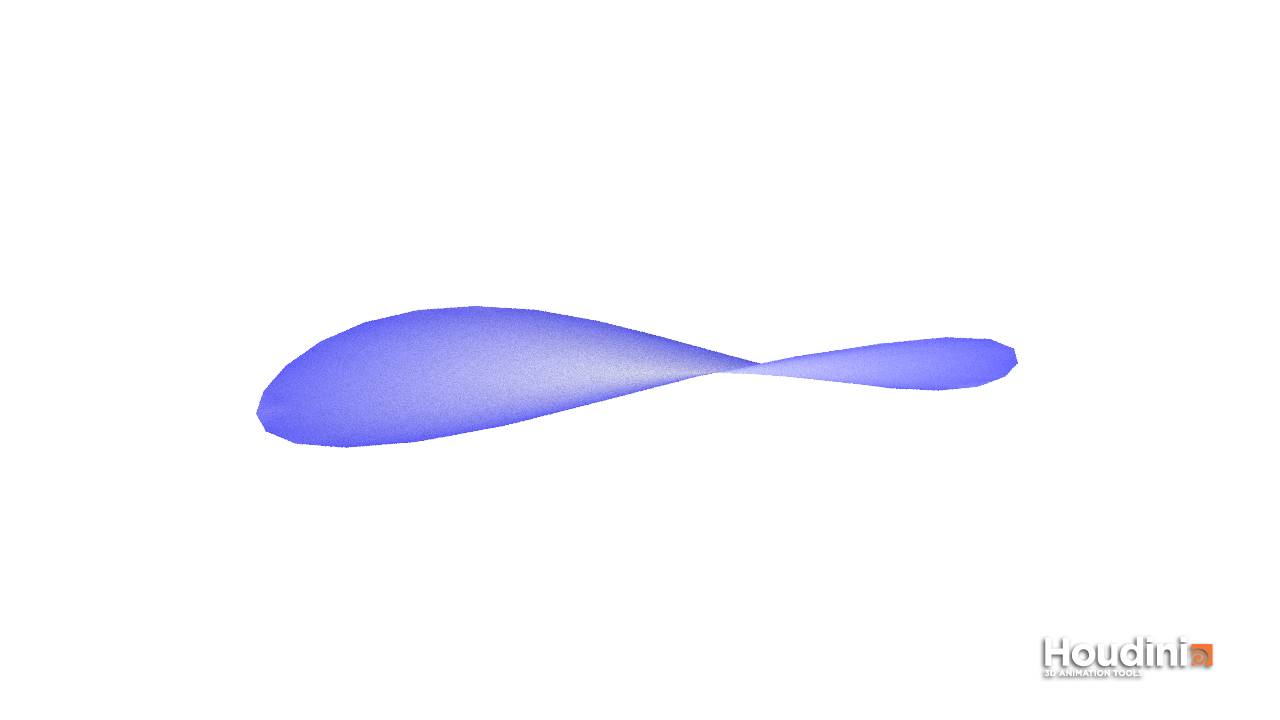
\includegraphics[width=\linewidth]{WetRimSim1.png} 
\caption{Caption1}
\label{fig:subim1}
\end{subfigure}%
\hfill
\begin{subfigure}{0.5\textwidth}
\centering
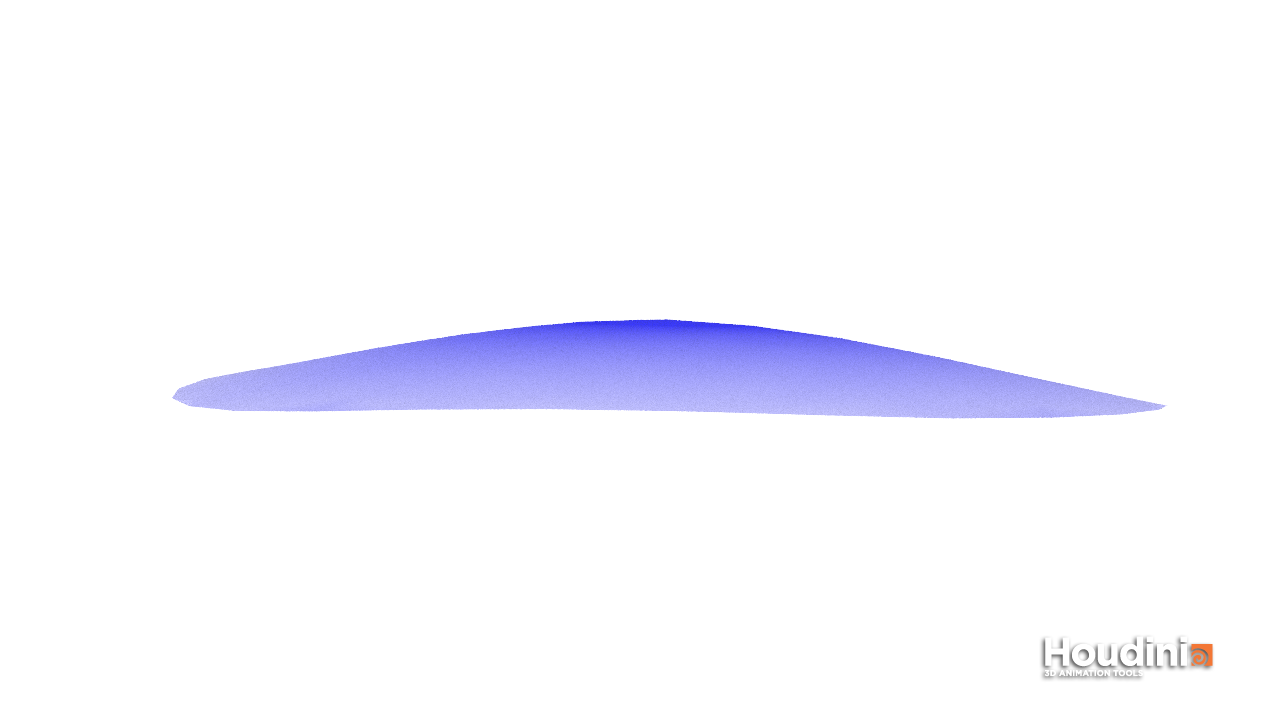
\includegraphics[width=\linewidth]{WetCenterSim2.png}
\caption{Caption 2}
\label{fig:WetDisc}
\end{subfigure}%

\end{figure}

\subsubsection{Machine Direction Experiment}
\begin{figure}[h]

\begin{subfigure}{0.45\textwidth}
\centering
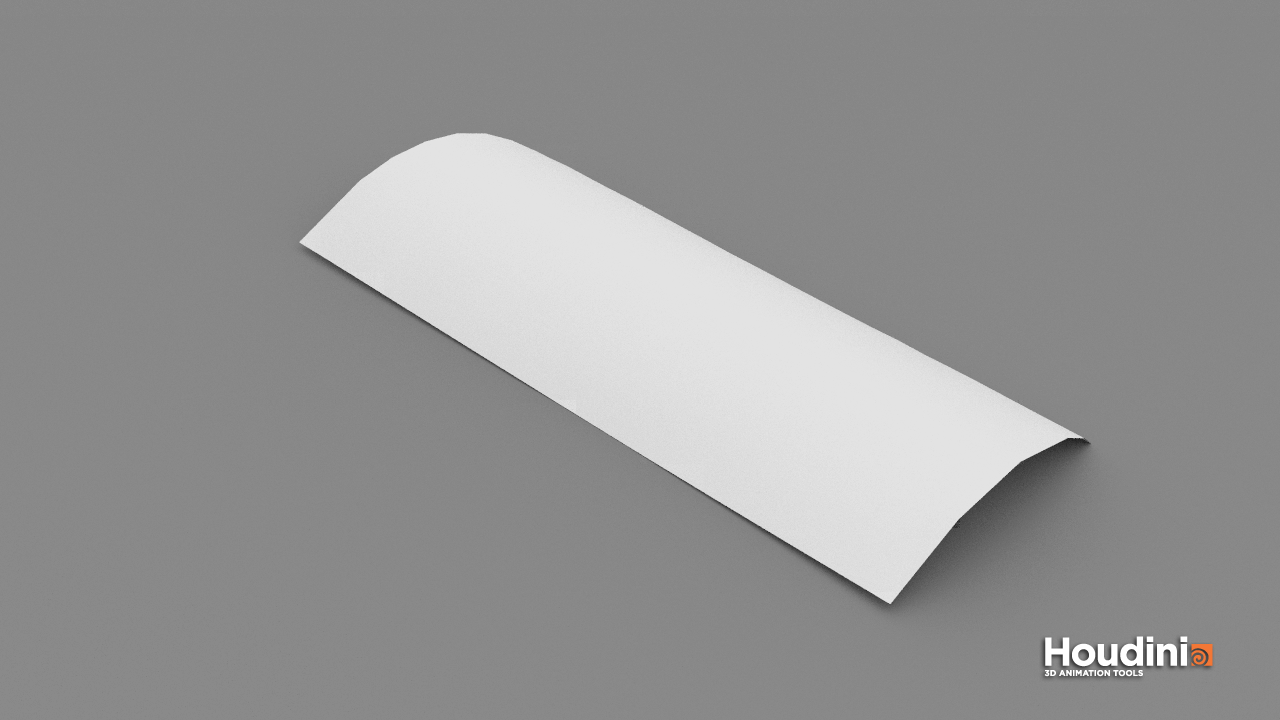
\includegraphics[width=\linewidth]{RechSim1.png} 
\caption{Caption1}
\label{fig:subim1}
\end{subfigure}%
\hfill
\begin{subfigure}{0.45\textwidth}
\centering
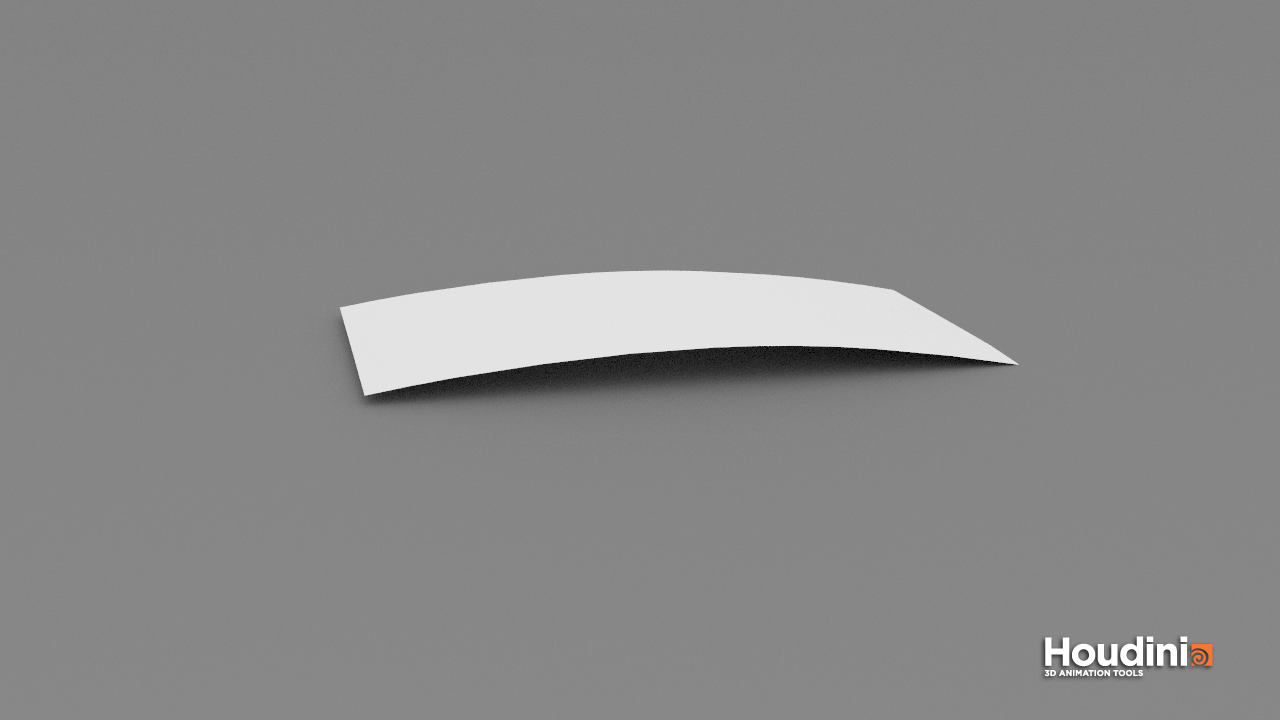
\includegraphics[width=\linewidth]{RecvSim1.png}
\caption{Caption 2}
\label{fig:Rec}
\end{subfigure}%

\end{figure}

\subsubsection{Dried Leaves}
\begin{figure}[h]
 
\begin{subfigure}{0.45\textwidth}
\centering
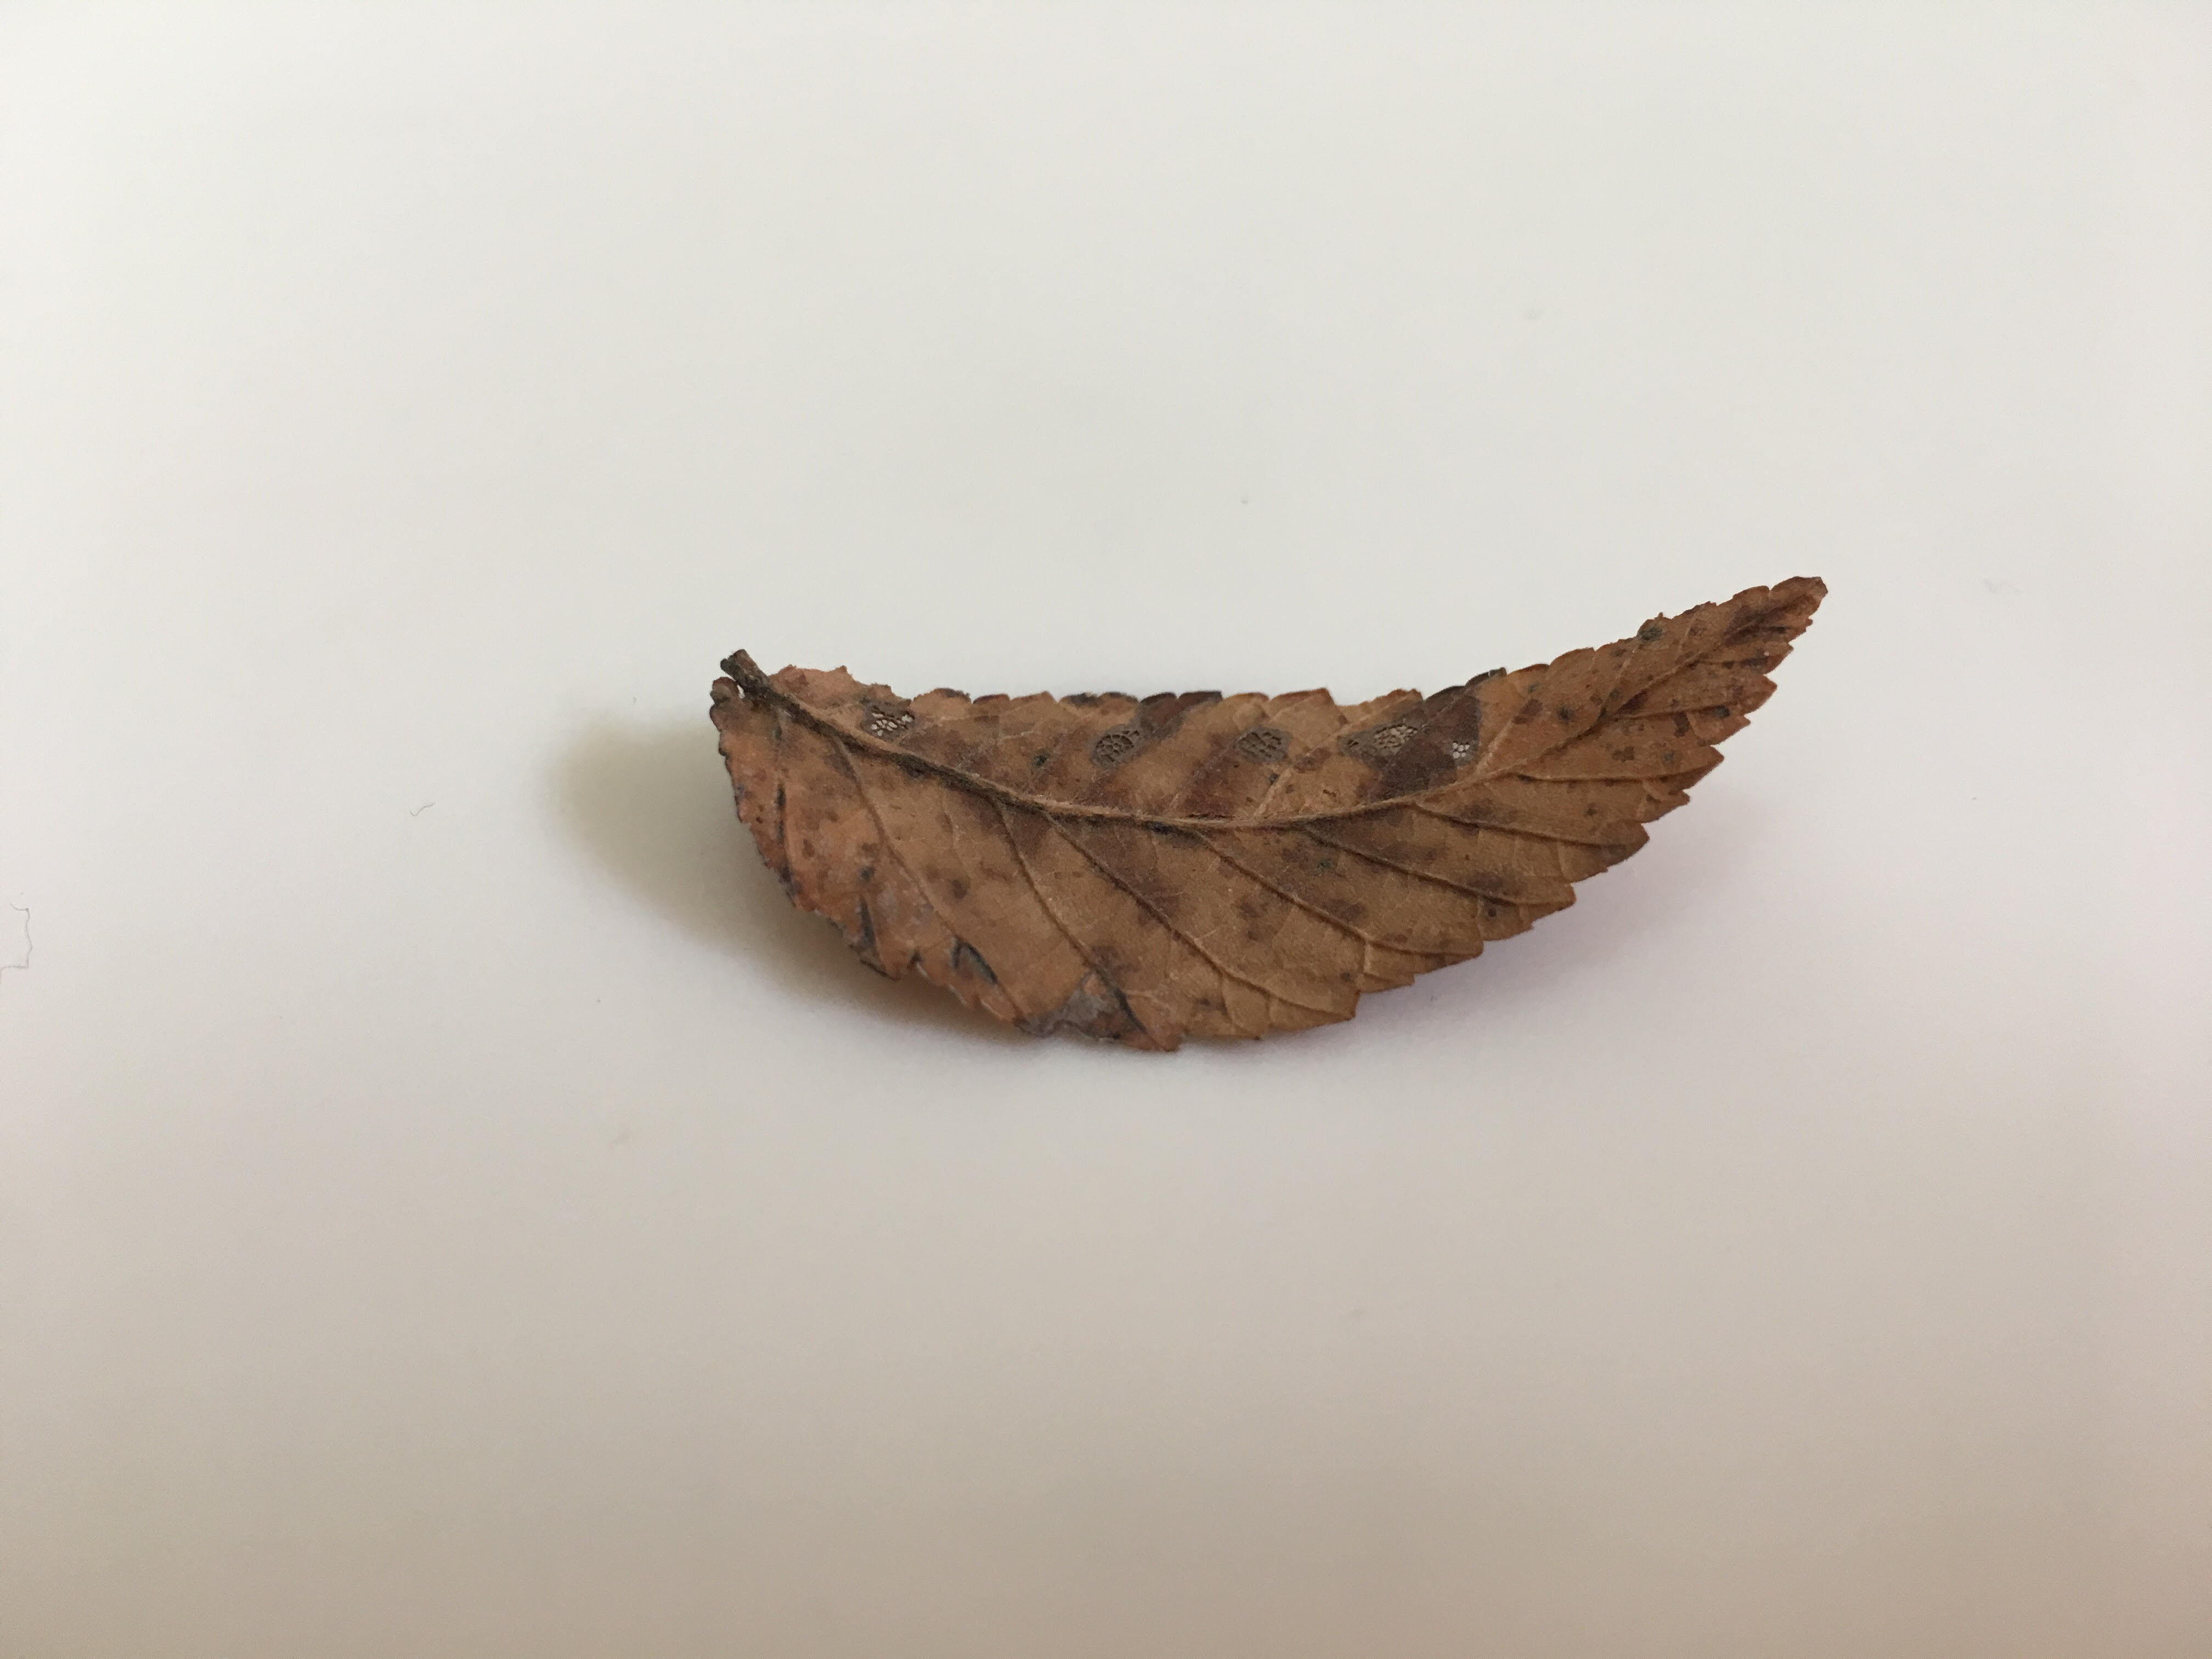
\includegraphics[width=0.45\linewidth]{actualLeafH2.jpg} 
\caption{Caption1}
\label{fig:subim1}
\end{subfigure}%
\hfill
\begin{subfigure}{0.45\textwidth}
\centering
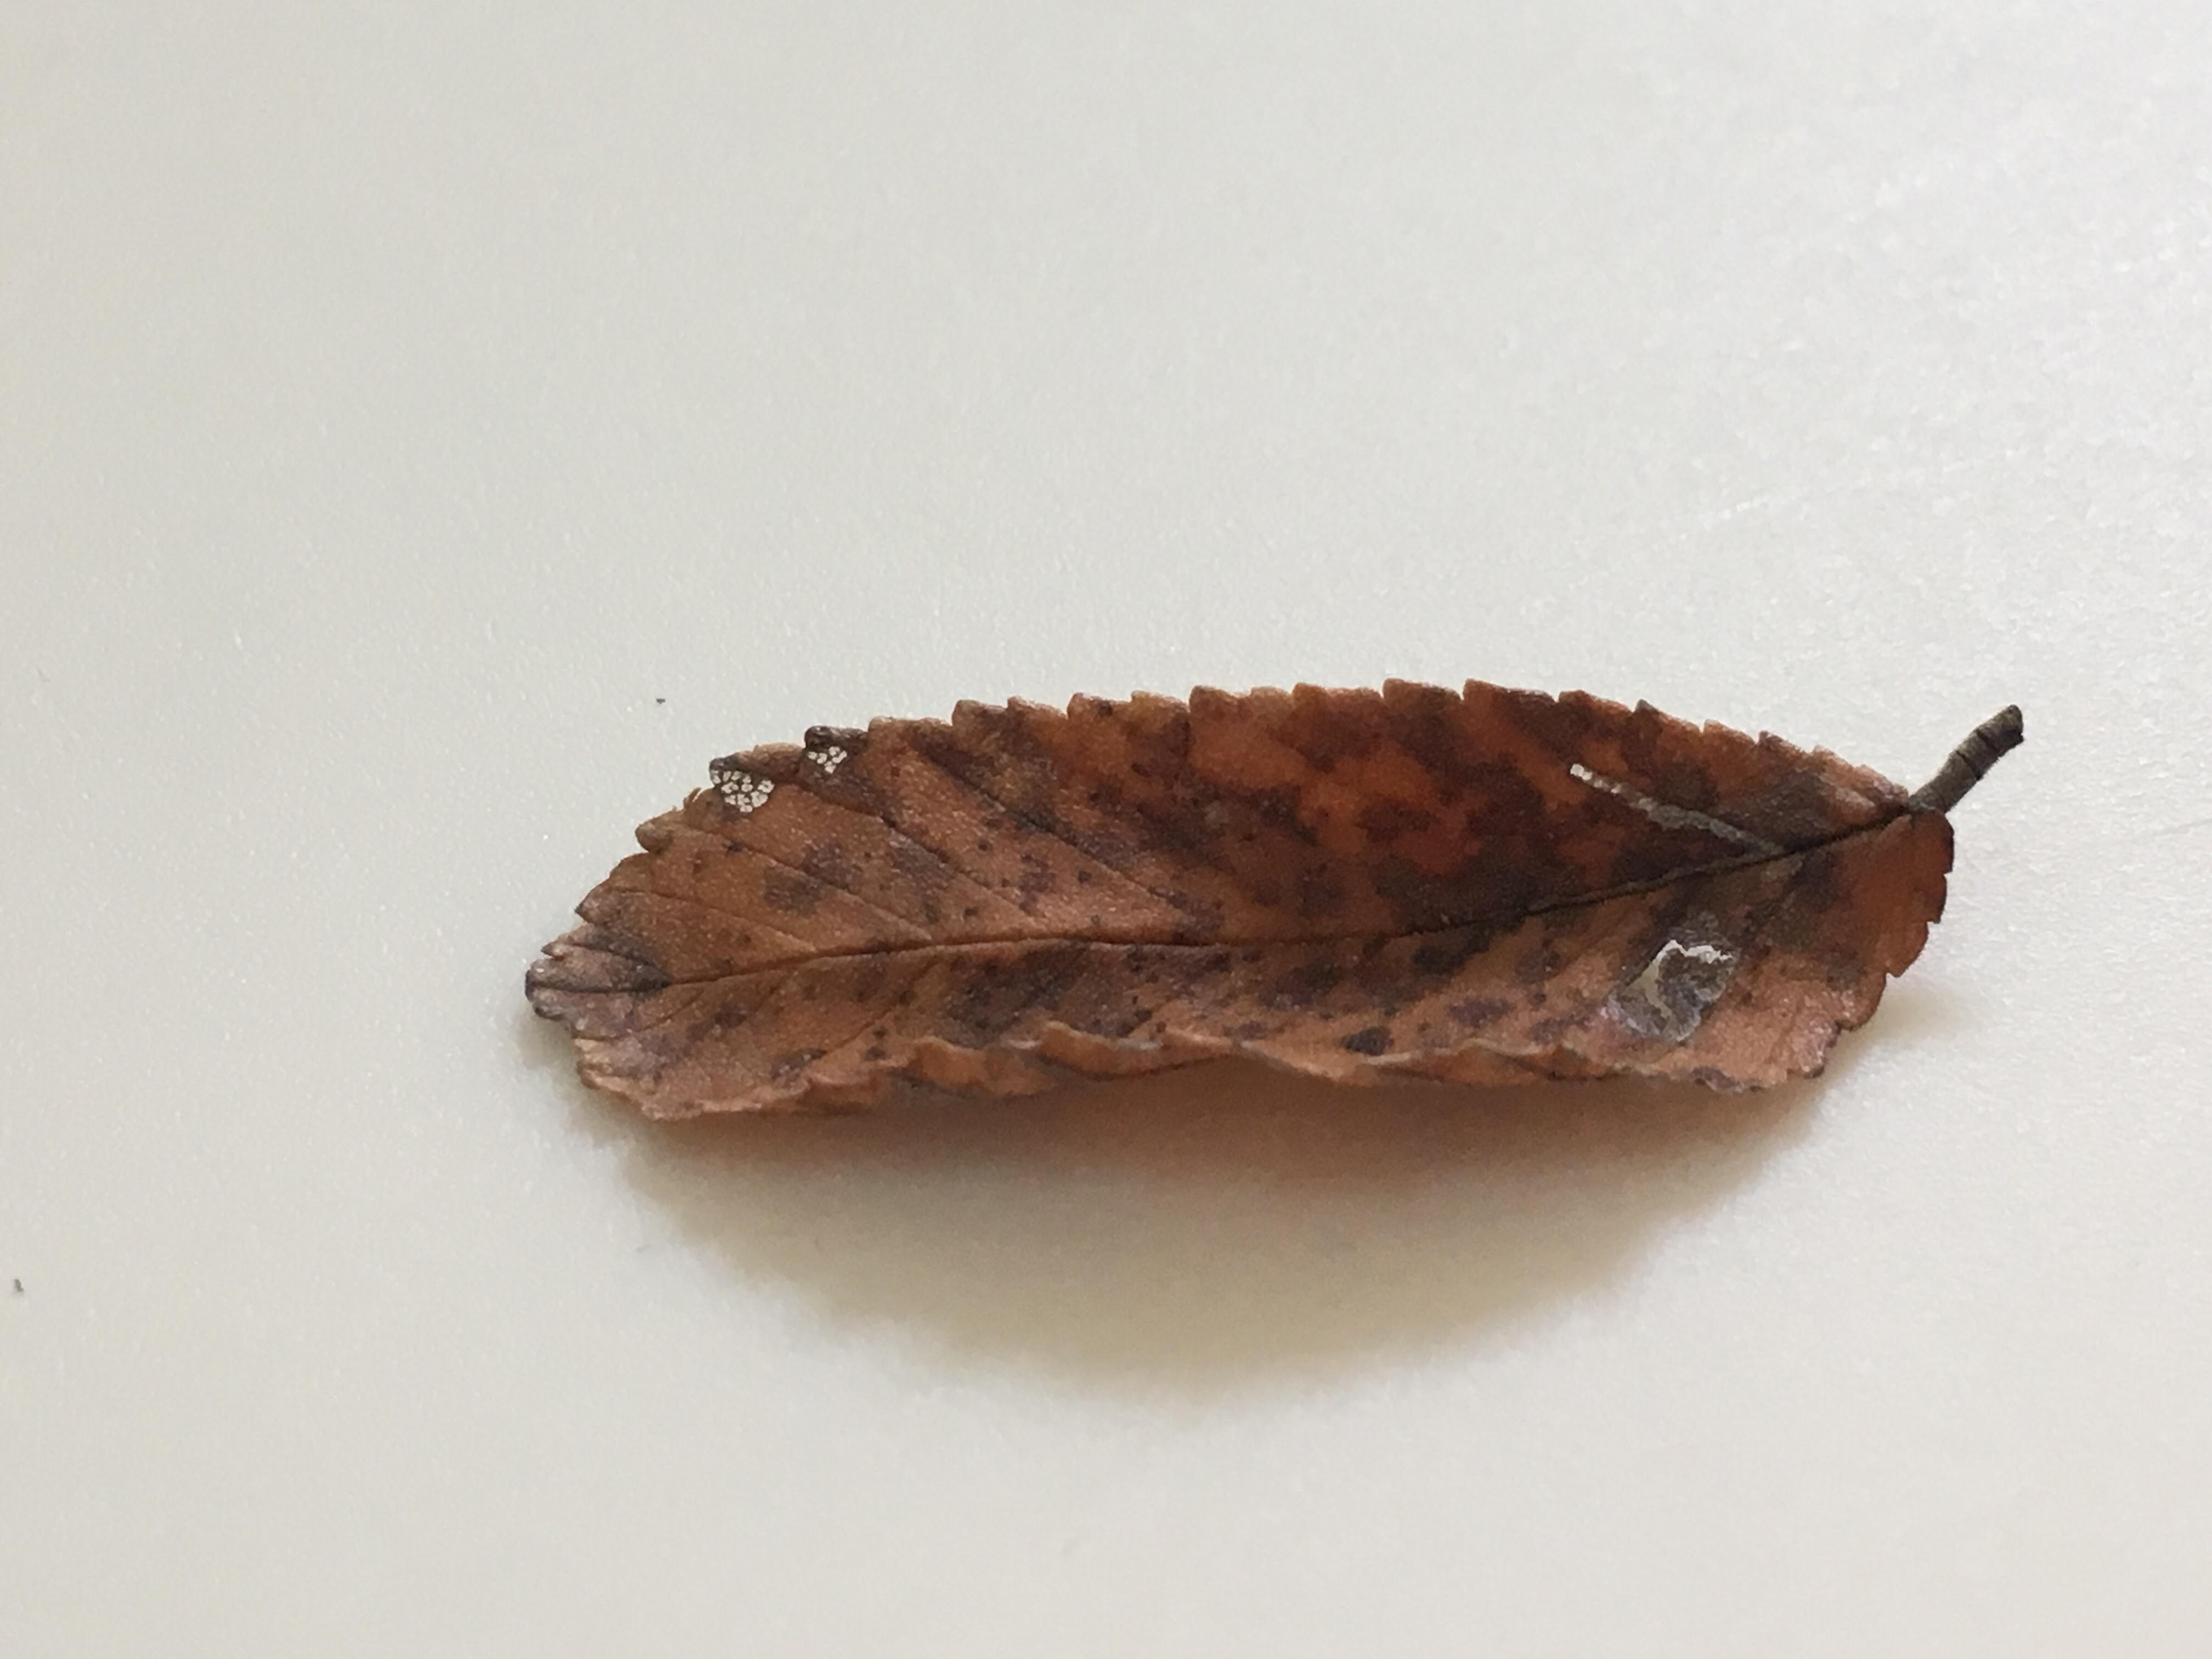
\includegraphics[width=0.45\linewidth]{actualLeafV.jpg}
\caption{Caption 2}
\label{fig:DriedLeaf}
\end{subfigure}%

\bigskip

\begin{subfigure}{0.45\textwidth}
\centering
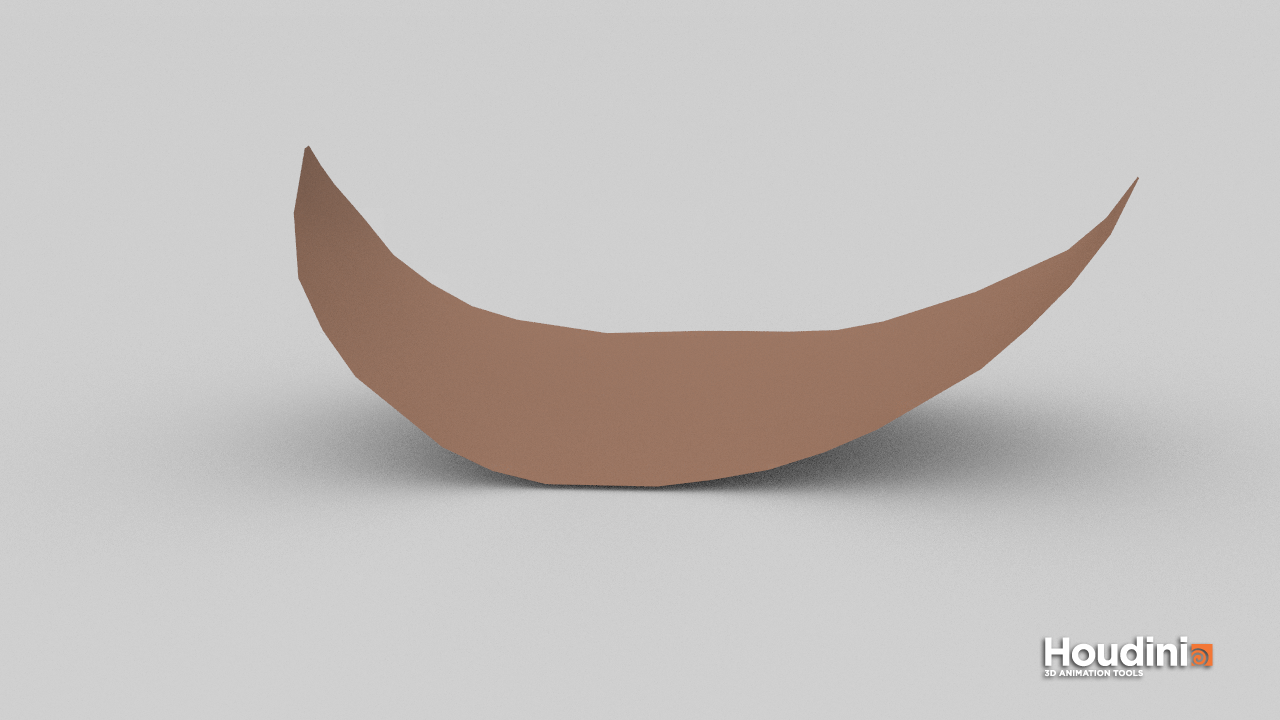
\includegraphics[width=0.45\linewidth]{LeafhSim1.png} 
\caption{Caption1}
\label{fig:subim3}
\end{subfigure}%
\hfill
\begin{subfigure}{0.45\textwidth}
\centering
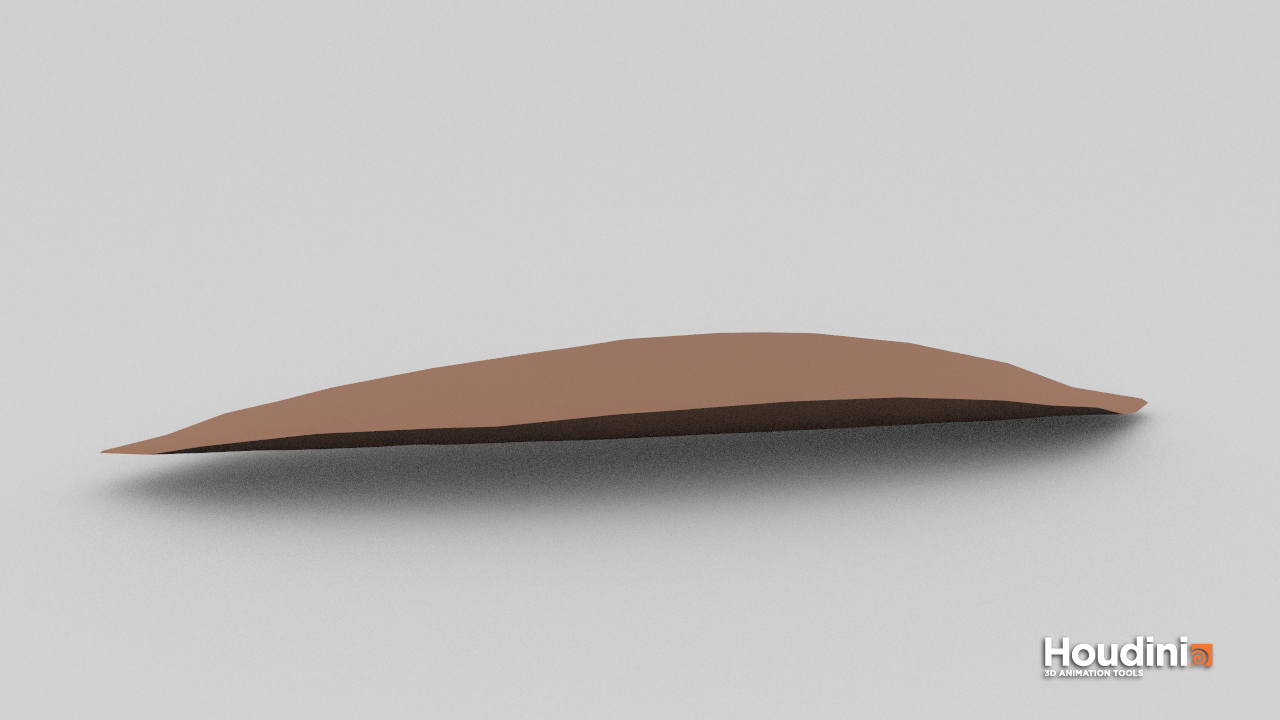
\includegraphics[width=0.45\linewidth]{LeafvSim1.png}
\caption{Caption 2}
\label{fig:subim4}
\end{subfigure}%
 
\caption{Simulation for Dried Leaves}
\label{fig:image2}
\end{figure}
\subsubsection{Wetting Paper Annulus}
\begin{figure}[h]
 
\begin{subfigure}{0.45\textwidth}
\centering
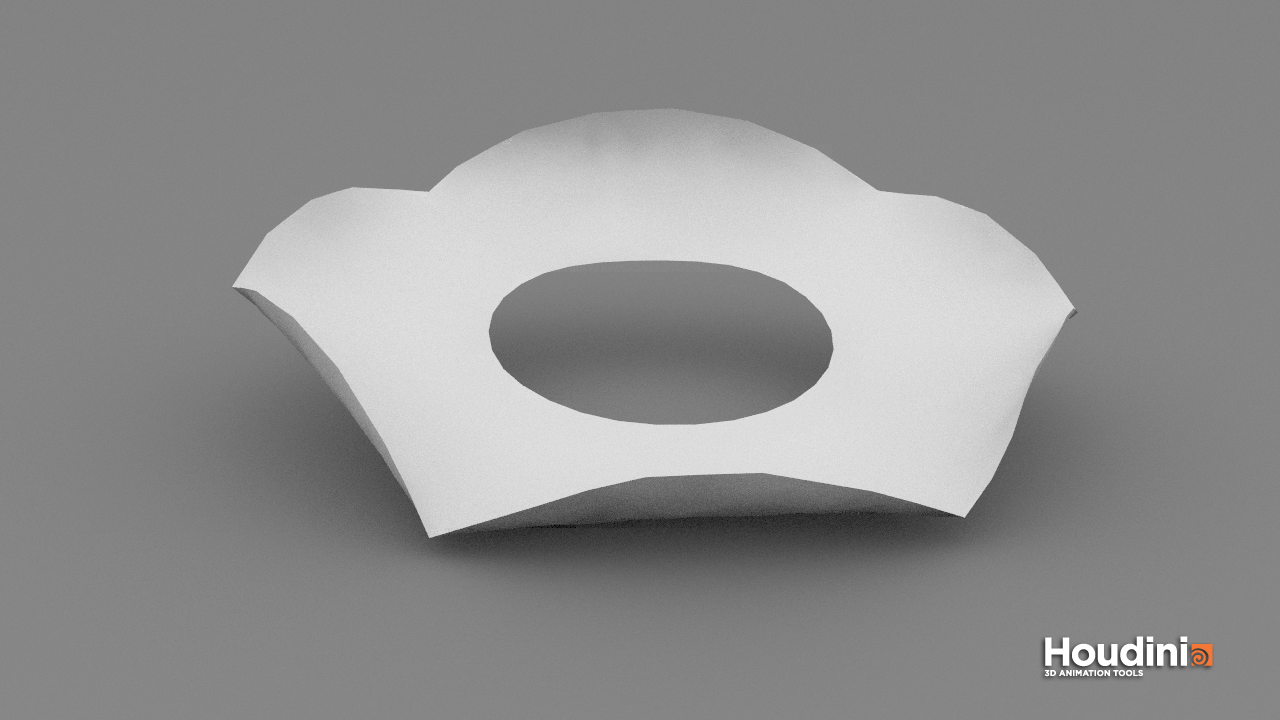
\includegraphics[width=0.45\linewidth]{AnnulusSim1.png} 
\caption{Caption1}
\label{fig:subim1}
\end{subfigure}%
\hfill
\begin{subfigure}{0.45\textwidth}
\centering
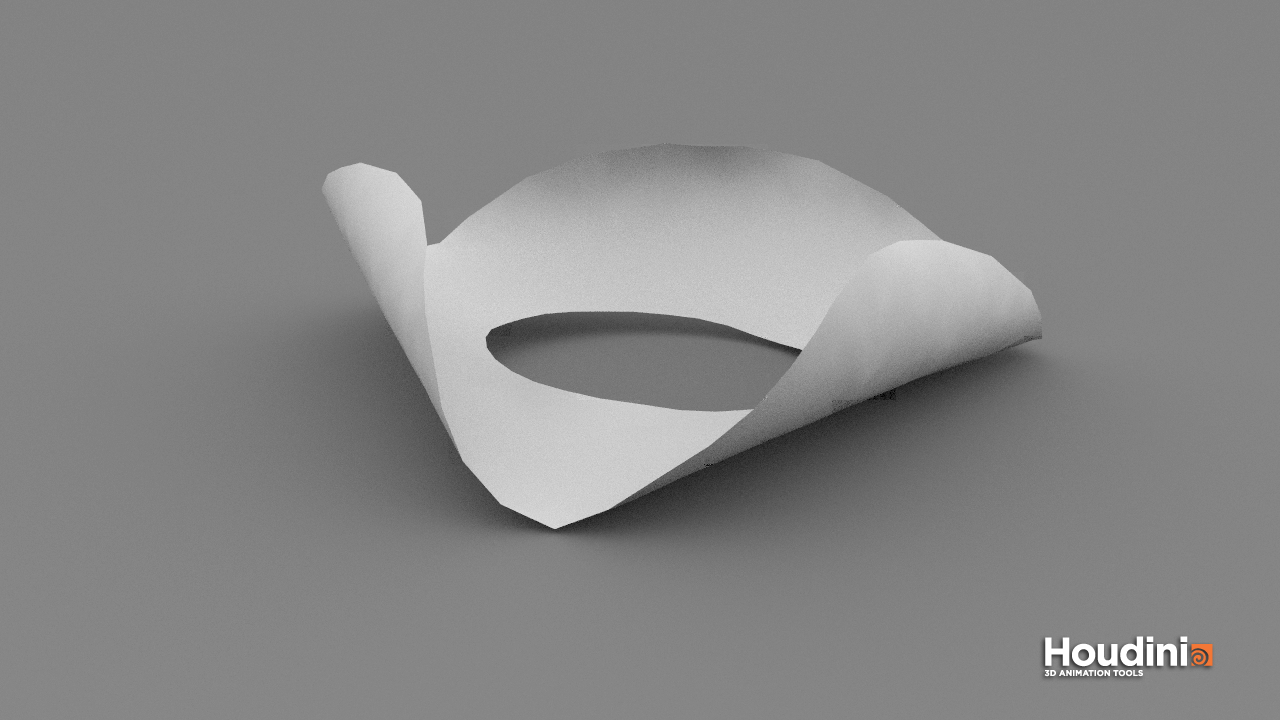
\includegraphics[width=0.45\linewidth]{AnnulusSim2.png}
\caption{Caption 2}
\label{fig:DriedLeaf}
\end{subfigure}%

\bigskip

\begin{subfigure}{0.45\textwidth}
\centering
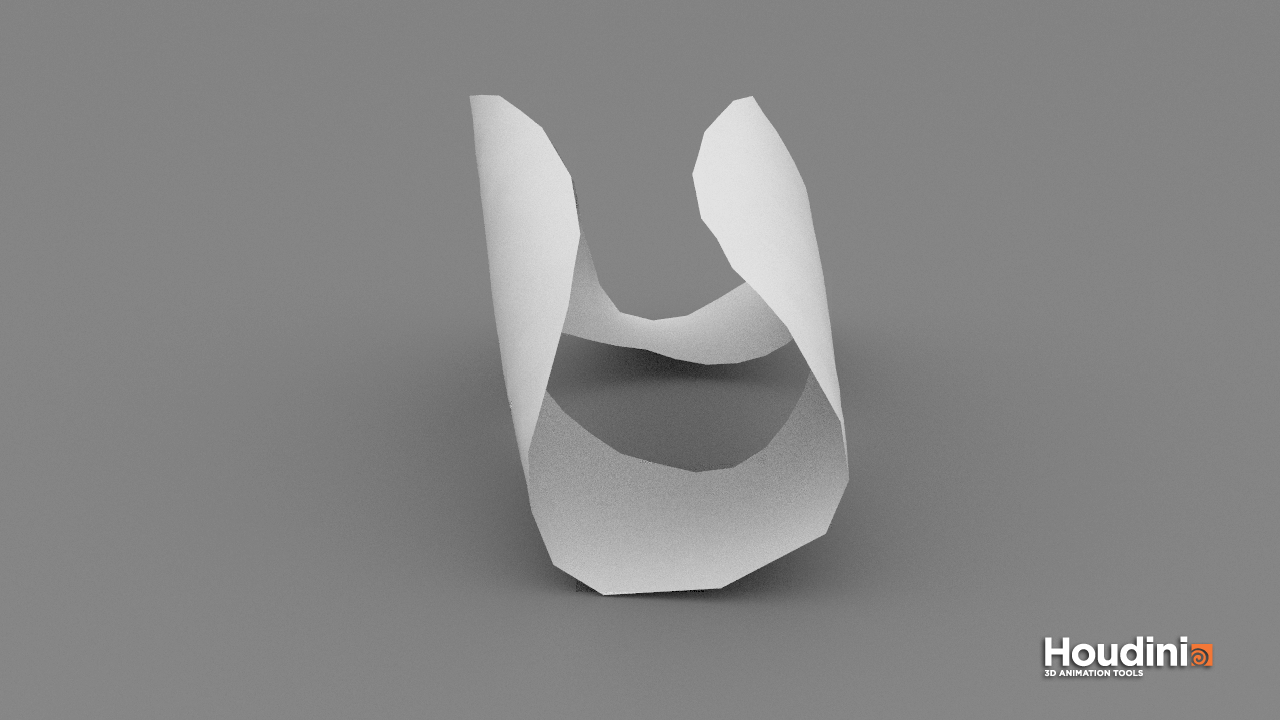
\includegraphics[width=0.45\linewidth]{AnnulusSim3.png} 
\caption{Caption1}
\label{fig:subim3}
\end{subfigure}%
 
\caption{Simulation for Wet Annulus}
\label{fig:image2}
\end{figure}

\subsubsection{Wetting Straw Wrapping Paper}
\subsubsection{Melting Spoon}
\subsubsection{Melting Torus}
\begin{figure}[h]
 
\begin{subfigure}{0.45\textwidth}
\centering
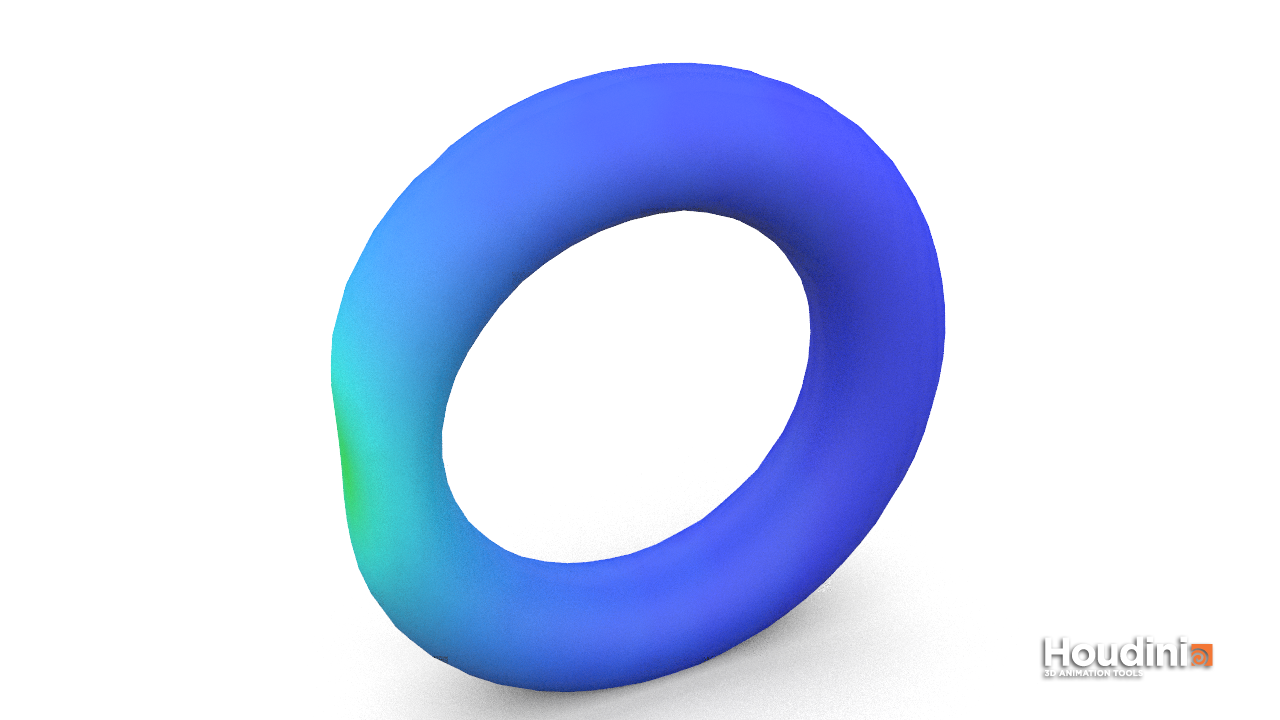
\includegraphics[width=0.45\linewidth]{TorusSim1.png} 
\caption{Caption1}
\label{fig:Torus1}
\end{subfigure}%
\hfill
\begin{subfigure}{0.45\textwidth}
\centering
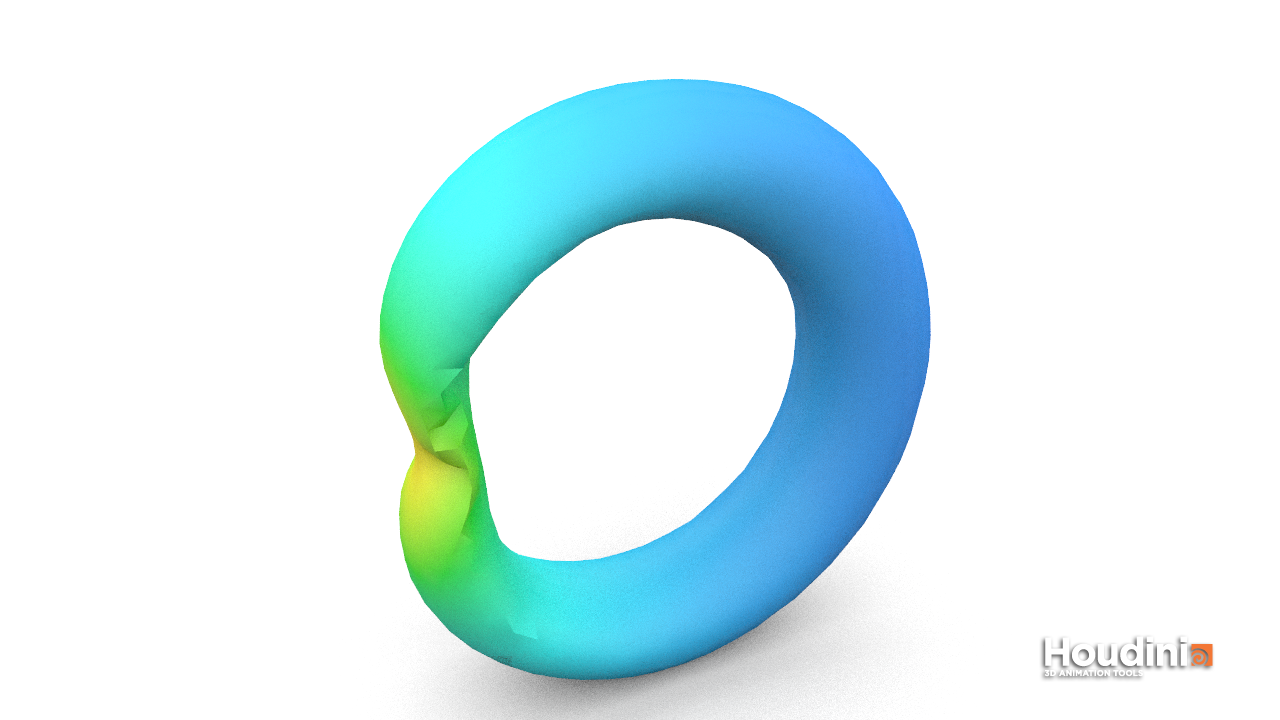
\includegraphics[width=0.45\linewidth]{TorusSim2.png}
\caption{Caption 2}
\label{fig:Torus2}
\end{subfigure}%

\bigskip

\begin{subfigure}{0.45\textwidth}
\centering
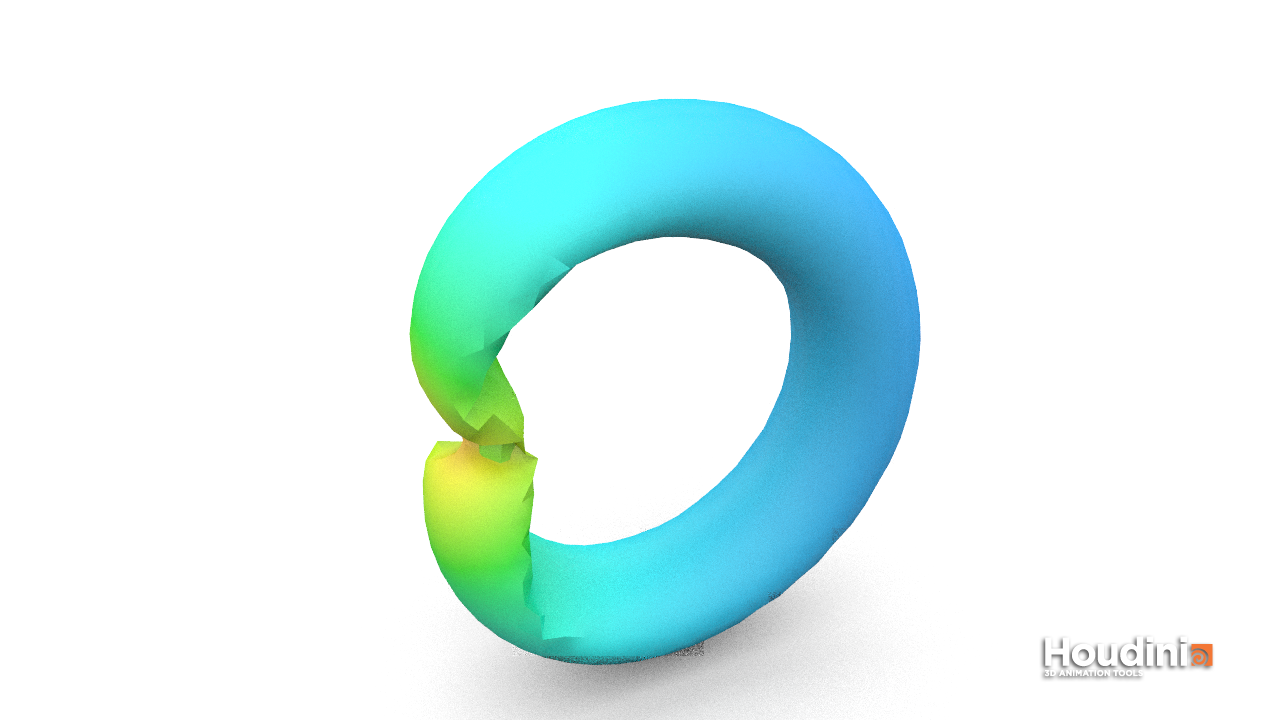
\includegraphics[width=0.45\linewidth]{TorusSim3.png} 
\caption{Caption1}
\label{fig:Torus3}
\end{subfigure}%
 
\caption{Simulation for Dried Torus}
\label{fig:Torus}
\end{figure}

\section{Conclusions and Future Work}

%Nullam vulputate enim ut tortor mollis pharetra. Cras pellentesque sem a accumsan malesuada. Donec at massa nisl. Sed malesuada felis id nisl maximus efficitur. In pretium metus non faucibus pulvinar. Sed pulvinar elit ultrices mauris vehicula, id ultricies purus finibus. Fusce tempus elit molestie, consequat ipsum eget, iaculis nibh. Cras tincidunt, orci in lacinia tempus, mauris leo finibus orci, vitae dignissim dui risus et odio. Sed commodo ultricies nulla, et varius velit aliquam quis. Sed efficitur, ex non facilisis dignissim, lacus orci accumsan massa, dictum facilisis arcu lacus ac leo. Sed quis tellus dictum massa egestas dapibus vel et justo. Nulla euismod lectus ut purus hendrerit porttitor. Suspendisse quis dui ligula. Proin non porta libero. Maecenas vel feugiat urna.
%
%\begin{acks}
%The authors would like to thank Dr. Yuhua Li for providing the MATLAB code of the \textit{BEPS} method.
%The authors would also like to thank the anonymous referees for their valuable comments and helpful suggestions. The work is supported by the \grantsponsor{GS501100001809}{National Natural Science Foundation of China}{https://doi.org/10.13039/501100001809} under Grant No.: ~\grantnum{GS501100001809}{61273304}
%21 and ~\grantnum[http://www.nnsf.cn/youngscientists]{GS501100001809}{Young Scientists' Support Program}.
%\end{acks}

\bibliographystyle{ACM-Reference-Format}
\bibliography{MoistSim}
\end{document}
